\section{问题二：缺失场景下的多模态情感预测模型}\label{sec:q2}

\subsection{问题分析与总体方案}\label{subsec:q2_plan}
局部连续缺失会使部分模态在统一序列中的一段时间没有可用观测，而文本、语音和视觉原本的有效位置仍需区分。问题二直接使用附件2已经预计算并对齐的三模态数值特征。本文以掩码均值池化和轻量时间注意力残差池化构成预测主干，图~\ref{fig:fig09_q2_model_architecture} 概括其结构；两个预测分支分别输出三类情感和连续强度。

模型结构由三条并行的单模态路径和一个共享预测部分构成。每条路径仅在有效时间位置聚合特征，均值表示经独立线性映射、层归一化、GELU及随机失活后，再与同一映射下的时间注意力表示作残差相加；三模态表示拼接后输入融合层，并连接分类和回归两个输出头。时间打分仅在各模态内部计算，填充位置在 softmax 前屏蔽。

该设计保留均值池化对整体上下文的概括，同时允许模型依据输入内容对局部时间位置赋予不同权重。残差系数以零初始化，使新增注意力分支开始时不改变基线表示；模态内打分则避免引入额外的跨模态交互假设。因而该结构以较少新增参数考察时间池化的作用，并保持分类与连续强度预测共享同一融合表示。

\begin{figure}[htbp]
  \centering
  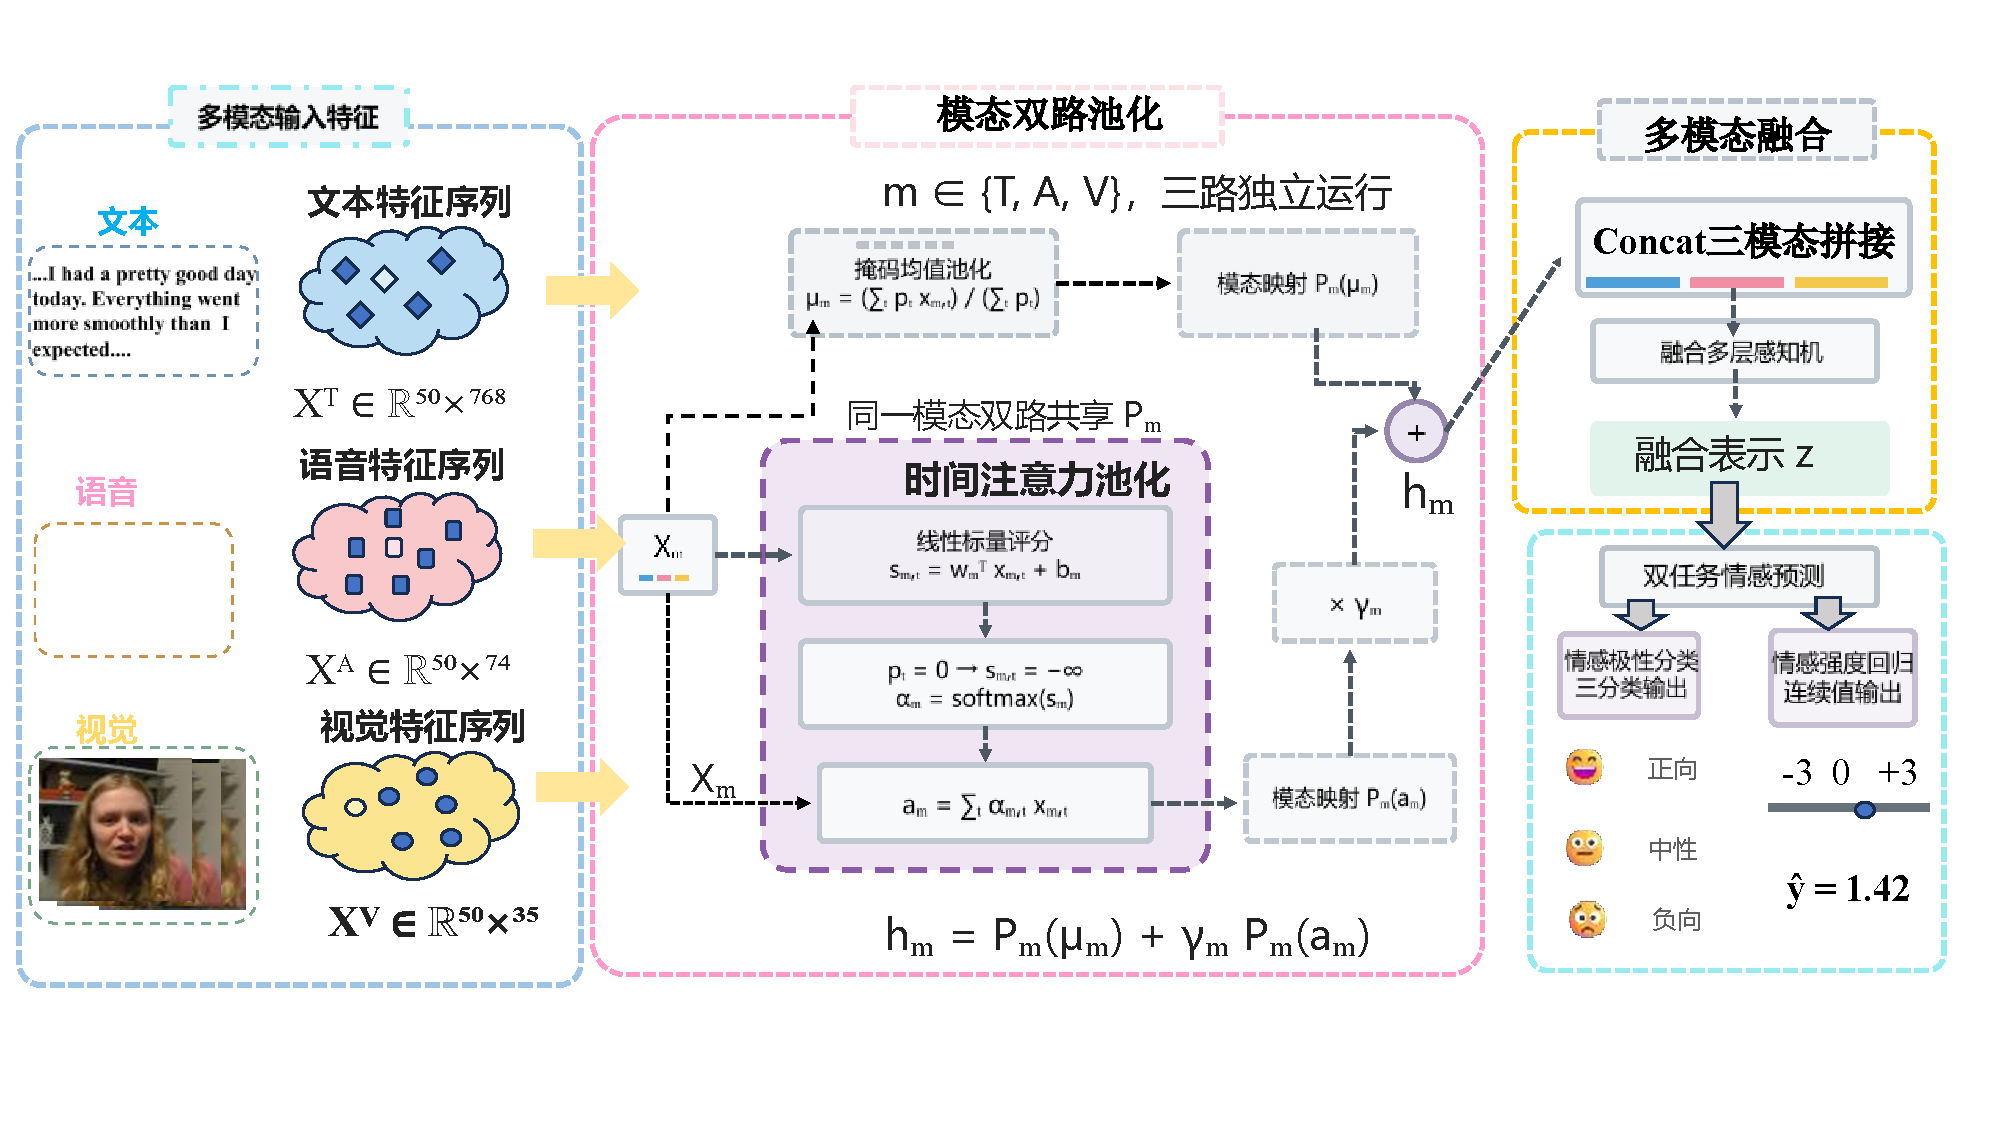
\includegraphics[width=1.0\textwidth]{figures/q2/fig09_q2_model_architecture.pdf}
  \caption{问题二的轻量时间注意力残差池化结构。三模态分别计算有效位置上的掩码均值与模态内时间注意力池化；共享模态映射后的残差表示经拼接融合，分别输出三类情感和连续强度。}
  \label{fig:fig09_q2_model_architecture}
\end{figure}

\subsection{数据表示与预测任务}\label{subsec:q2_data}
附件2的训练、验证和测试划分分别包含3395、728和727条样本。每条样本的文本、语音和视觉特征长度均为50，特征维数依次为768、74和35。本文仅利用训练集拟合参数，使用验证集进行模型确定、三次随机初始化比较及缺失场景分析；附件2测试划分不参与上述选择与结论。附件3为无标签推理数据，不参与本节评价。

记 $p_{it}\in\{0,1\}$ 为样本 $i$ 在位置 $t$ 的有效位。该掩码依据附件中的 \texttt{text\_bert[:,1,:]} 有效位字段构造；经数据审计，三模态在文本填充区间之外没有非零特征。有效位置中的原生全零向量仍保留在观测序列内。另设观测可用性掩码，仅在构造人工缺失时把指定连续区间置为不可用；模型不把该掩码作为额外输入。三分类按连续标注的负值、零值和正值分别对应消极、中性和积极，并沿用附件给出的实际类别编码。

图~\ref{fig:fig10_q2_data_statistics} 描述附件2各划分规模，并展示训练集和验证集的三分类标签、连续情感强度及有效序列长度。训练集与验证集的积极类均为多数类、中性类样本相对较少，这一分布构成采用训练集频数计算平衡加权交叉熵的背景；有效长度从3至50个时间位置不等，说明池化时需显式屏蔽填充位置。图中测试集只显示样本数，其标签未用于此处统计；这些描述性分布不用于推断模型泛化性能。

\begin{figure}[!htbp]
  \centering
  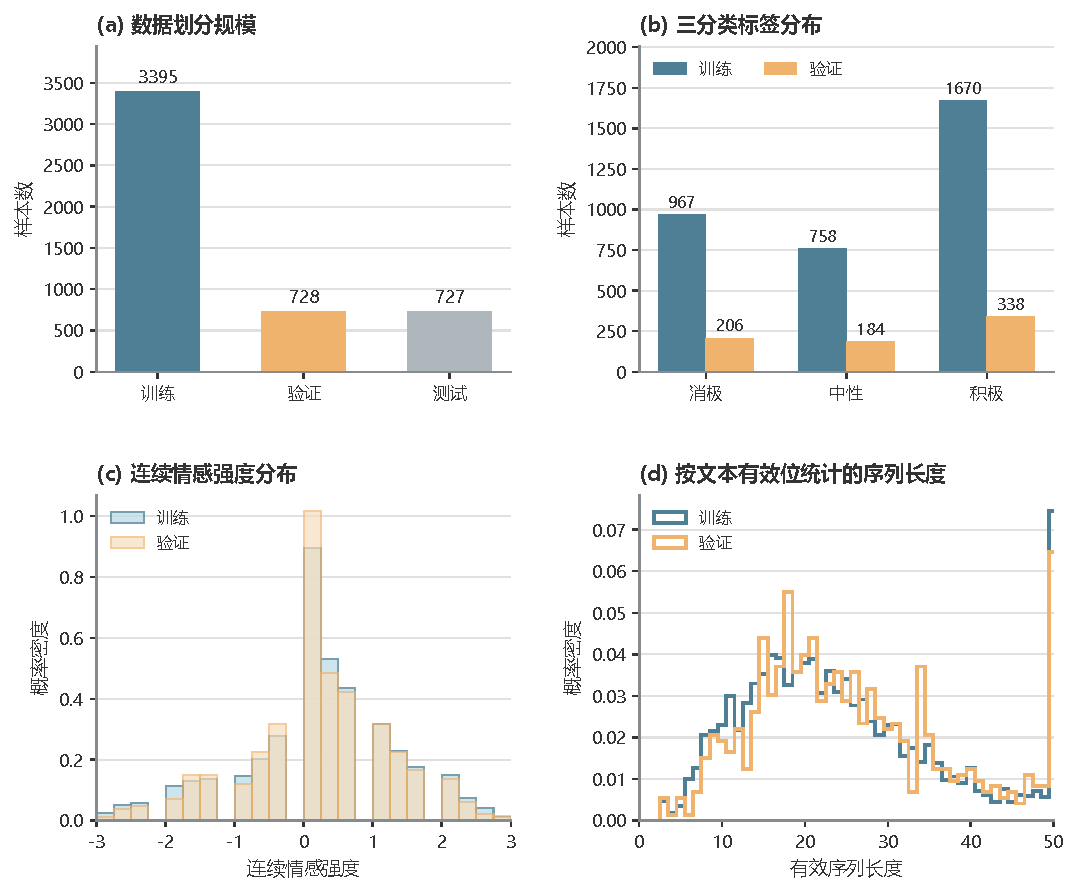
\includegraphics[width=0.98\textwidth]{figures/q2/fig10_q2_data_statistics.pdf}
  \caption{附件2 aligned-50 特征的数据划分与标签统计。(a) 训练、验证和测试划分的样本规模；(b) 训练集与验证集的三分类标签分布；(c) 连续情感强度分布；(d) 根据文本有效位字段统计的有效序列长度分布。测试划分仅展示样本数量，不参与标签统计、模型选择或性能分析。}
  \label{fig:fig10_q2_data_statistics}
\end{figure}
\FloatBarrier

\subsection{基线多模态情感预测模型}\label{subsec:q2_base}
基线模型对各模态分别进行有效位置上的均值池化，然后以独立映射将每个模态压缩至128维。对样本 $i$ 的模态 $m$，定义
\begin{equation}
\boldsymbol\mu_i^{(m)}
=\frac{\sum_{t=1}^{50}p_{it}\mathbf x_{it}^{(m)}}{\sum_{t=1}^{50}p_{it}},
\qquad
\mathbf h_{i,0}^{(m)}=P_m\!\left(\boldsymbol\mu_i^{(m)}\right),
\label{eq:q2_mean}
\end{equation}
其中 $P_m$ 依次包含线性映射、层归一化、GELU和随机失活。原生零向量只要位于有效位置，就按原值参与式~\eqref{eq:q2_mean}。三个128维表示拼接为384维，经128维融合层后送入三分类分支与单值回归分支。基线模型共有163460个参数。

分类采用仅由训练集类别频数确定的平衡加权交叉熵，$w_c=N/(3N_c)$；回归采用SmoothL1损失。总目标为
\begin{equation}
\mathcal L=\mathcal L_{\mathrm{WCE}}+\lambda_{\mathrm r}\mathcal L_{\mathrm{SmoothL1}},
\qquad \lambda_{\mathrm r}=1.
\label{eq:q2_loss}
\end{equation}
输入不作默认标准化，也不在训练时加入人工连续缺失。优化采用AdamW，学习率$10^{-3}$、权重衰减$10^{-4}$、批量大小128，随机失活率0.1；最多训练80轮，提前停止耐心轮数为12。这些设定对应实际实验配置，未依据附件2测试划分调整。

\subsection{轻量时间注意力残差池化模型}\label{subsec:q2_pool}
均值池化对有效位置赋予相同权重，可能削弱短暂但关键的情绪线索。为补充时间维度信息，本文对每一模态增加一个标量打分器，并在有效位置上归一化：
\begin{equation}
e_{it}^{(m)}=f_m(\mathbf x_{it}^{(m)}),\quad
\alpha_{it}^{(m)}
=\frac{p_{it}\exp(e_{it}^{(m)})}{\sum_{s:p_{is}=1}\exp(e_{is}^{(m)})},\quad
\mathbf a_i^{(m)}=\sum_{t=1}^{50}\alpha_{it}^{(m)}\mathbf x_{it}^{(m)} .
\label{eq:q2_attention}
\end{equation}
填充位置在归一化前屏蔽，因此其注意力权重为零。时间表示使用与均值路径相同的模态映射，最终表示为
\begin{equation}
\mathbf h_i^{(m)}
=P_m(\boldsymbol\mu_i^{(m)})
+\gamma_mP_m(\mathbf a_i^{(m)}).
\label{eq:q2_residual}
\end{equation}
三个残差系数初始为零，使模型初始预测与相应基线完全一致。改进模型保持已确定的模态映射、融合层和预测分支参数不变，仅估计新增的模态打分器及残差系数，使性能变化集中于池化方式。新增可调参数为883个，约为基线参数量的0.54\%；总参数量为164343。该结构不使用跨模态注意力或额外的重建网络。

\subsection{缺失场景构造与鲁棒性评价}\label{subsec:q2_benchmark}
评估协议由完整输入和54个预定的连续缺失场景组成。单模态场景对文本、语音或视觉分别设置$\rho\in\{0.1,0.2,0.3,0.4,0.5\}$，并在有效前缀的前段、中段和后段放置遮挡，共45种。双模态场景取文本与语音、文本与视觉、语音与视觉三种组合，统一使用$\rho=0.3$及三个位置，共9种。若有效长度为$L_i$，遮挡长度为$\ell_i=\max(1,\operatorname{round}(\rho L_i))$；三个起点依次为$0$、$\lfloor(L_i-\ell_i)/2\rfloor$和$L_i-\ell_i$。人工缺失在模型输入中覆盖为精确零向量，填充区间与原生零记录均不因此改写。各模型使用相同的预定场景定义。

完整输入与各缺失条件均报告准确率、宏平均F1、平均绝对误差（MAE）和皮尔逊相关系数。为在开发验证中同时兼顾分类与回归，另定义内部综合分数
\begin{equation}
S=\tfrac14\operatorname{Acc}+\tfrac14\operatorname{MacroF1}
+\tfrac14(1-\operatorname{MAE}/6)
+\tfrac18(\operatorname{Pearson}+1),\qquad
R=\tfrac12\!\left(S_{\mathrm{clean}}+\frac1{54}\sum_{j=1}^{54}S_j\right).
\label{eq:q2_score}
\end{equation}
$R$仅为本项目的验证比较指标，不是竞赛官方评分。基线参数按完整输入验证分数确定，改进模型按预定的$R$确定；比较时保留这一选择口径差异。图~\ref{fig:fig11_q2_missing_ratio} 和图~\ref{fig:fig12_q2_missing_location} 分别用于展示比例变化与模态/位置组合。

\begin{figure}[htbp]
  \centering
  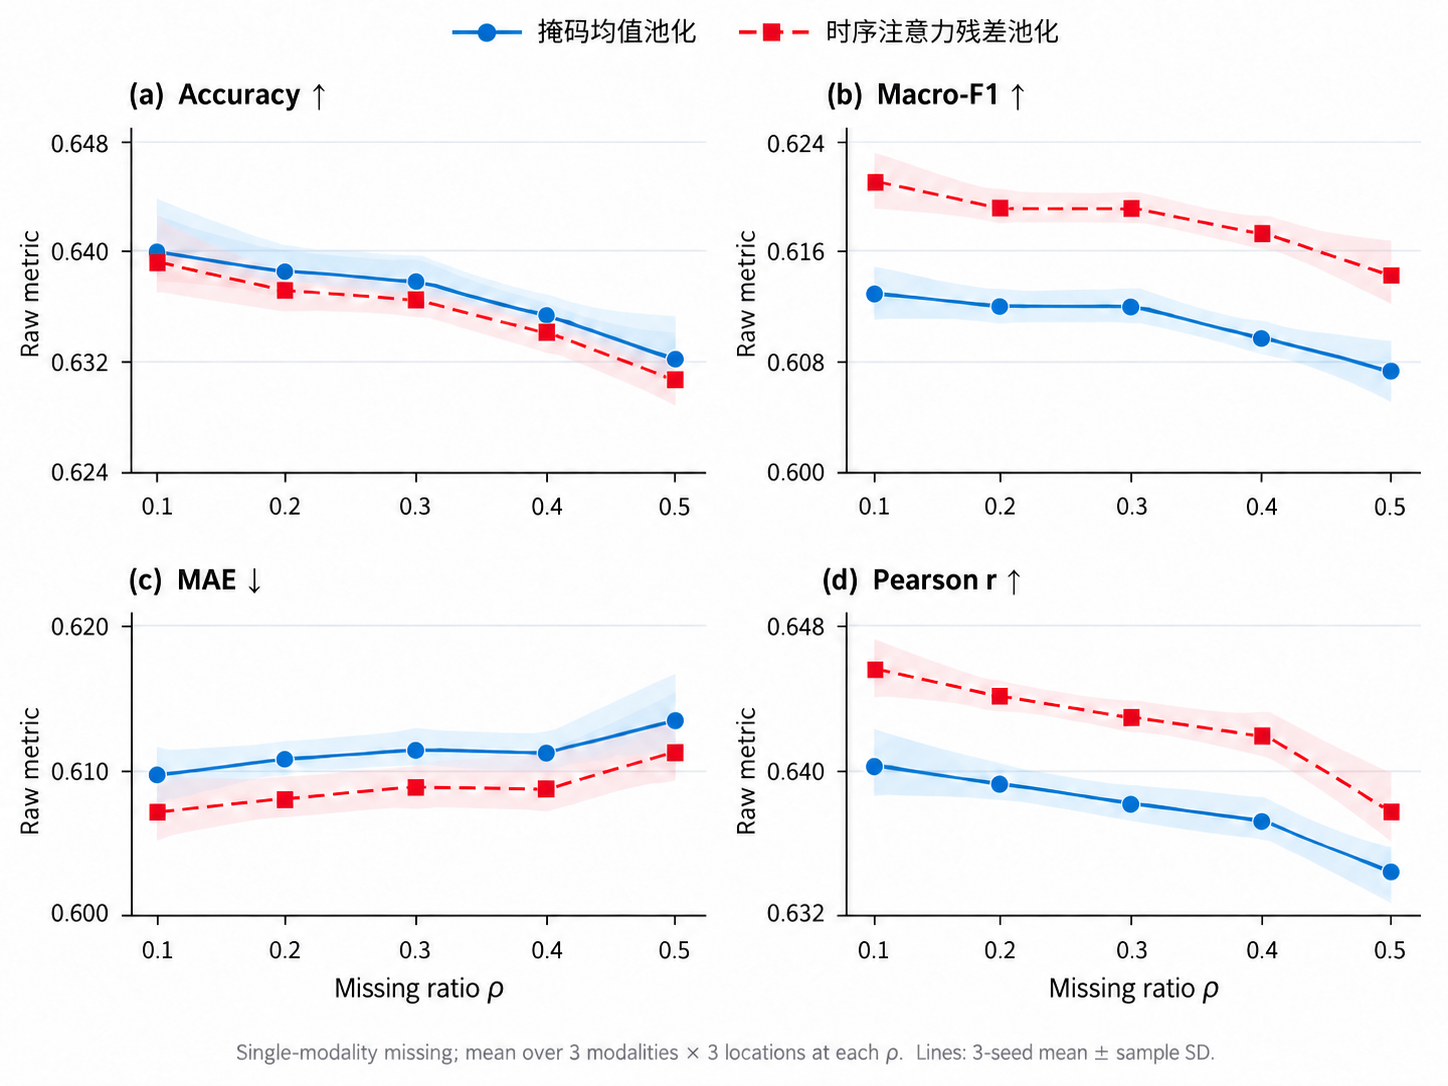
\includegraphics[width=1.0\textwidth]{figures/q2/fig11_q2_missing_ratio_four_metrics.png}
  \caption{不同单模态连续缺失比例下的验证集性能。每个比例先对三种模态与前、中、后三种遮挡位置取平均，再绘制三次随机初始化的均值与样本标准差；阴影为样本标准差。蓝线为掩码均值池化基线，红线为时间注意力残差池化模型；MAE 越低越好，其余指标越高越好。}
  \label{fig:fig11_q2_missing_ratio}
\end{figure}

\begin{figure}[htbp]
  \centering
  % TODO: replace with final figure
  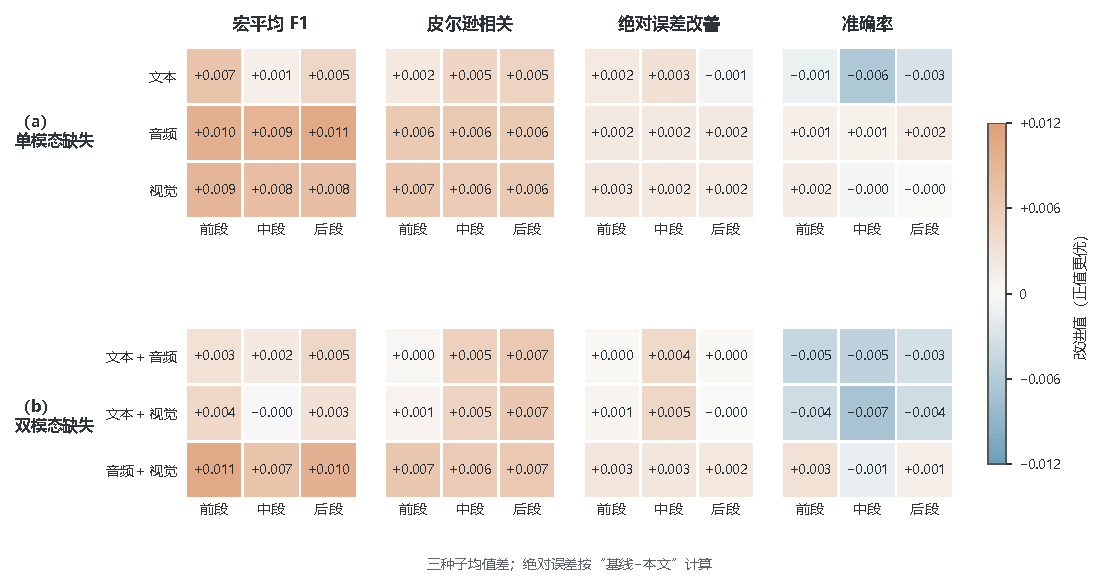
\includegraphics[width=1.0\textwidth]{figures/q2/fig12_q2_missing_location_modality_stress.pdf}
  \caption{缺失模态及位置对模型间性能差异的影响。宏平均F1、相关系数和准确率为“本文模型减基线模型”，MAE为“基线模型减本文模型”，故正值均表示本文模型较优；色块为验证集三次随机初始化均值之差。}
  \label{fig:fig12_q2_missing_location}
\end{figure}

\subsection{实验结果与分析}\label{subsec:q2_results}
\subsubsection{完整输入与平均缺失条件}
表~\ref{tab:q2_main} 给出三次随机初始化的验证集均值及样本标准差。完整输入下，本文模型的宏平均F1由0.6139增至0.6241，MAE由0.6079降至0.6059；平均缺失条件下，宏平均F1由0.6092增至0.6163，MAE由0.6111降至0.6091，相关系数由0.6359增至0.6414。与此同时，平均缺失准确率从0.6349略降为0.6340。这些结果支持小幅平均改进，不支持所有指标均改善的表述。

\begin{table}[htbp]
\centering\small
\caption{附件2验证集上完整输入与54种缺失条件的预测结果（三次随机初始化均值$\pm$样本标准差）}
\label{tab:q2_main}
\begin{tabular}{@{}llcccc@{}}
\toprule
模型 & 条件 & 准确率$\uparrow$ & 宏平均F1$\uparrow$ & MAE$\downarrow$ & 相关系数$\uparrow$\\
\midrule
基线模型 & 完整 & $0.6401\pm0.0048$ & $0.6139\pm0.0091$ & $0.6079\pm0.0103$ & $0.6409\pm0.0043$\\
本文模型 & 完整 & $0.6419\pm0.0057$ & $0.6241\pm0.0026$ & $0.6059\pm0.0066$ & $0.6472\pm0.0025$\\
\addlinespace
基线模型 & 平均缺失 & $0.6349\pm0.0062$ & $0.6092\pm0.0075$ & $0.6111\pm0.0098$ & $0.6359\pm0.0038$\\
本文模型 & 平均缺失 & $0.6340\pm0.0049$ & $0.6163\pm0.0012$ & $0.6091\pm0.0060$ & $0.6414\pm0.0025$\\
\bottomrule
\end{tabular}
\end{table}

\subsubsection{缺失比例、模态与位置}
不同遮挡比例的分组结果如图~\ref{fig:fig11_q2_missing_ratio} 所示。随着缺失范围扩大，两个模型的内部综合分数整体下降；在比例0.5的分组中，本文模型与基线模型的平均综合分数分别为0.7392与0.7372。图~\ref{fig:fig12_q2_missing_location} 进一步显示，收益依赖模态和缺失位置：18个模态/位置组合中，宏平均F1有17个均值差为正，相关系数有18个为正，MAE改善有16个为正，而准确率仅6个为正。该方向计数不表示每次随机初始化或每个样本均受益。文本与语音、文本与视觉同时缺失时，综合收益接近零，说明关键模态同时失去观测后，简单池化残差的补偿能力有限。

\subsubsection{随机初始化稳定性与误差分析}
三次对应初始化下，本文模型相对基线模型的综合鲁棒分数差依次为$+0.005600$、$+0.003791$和$-0.000090$，平均为$+0.003100\pm0.002907$（样本标准差）。两次获得正向改进，一次基本持平，表明改进具有一定初始化敏感性。图~\ref{fig:fig13_q2_stability_error_analysis}(a)给出相同种子下的配对分数；(b)展示种子42的干净验证集混淆矩阵，便于观察中性类的识别差异；(c)汇总不同缺失场景的选择分数；(d)单独呈现视觉整段原生全零子集。基线与本文模型的鲁棒分数均值分别为$0.741677\pm0.001458$和$0.744777\pm0.001492$。验证集中有15个视觉整段原生全零样本，保留该子集及原标签后观察到部分初始化下本文模型在该子集的分类表现低于基线，因此不能用总体均值掩盖这一局部风险。

\begin{figure}[htbp]
  \centering
  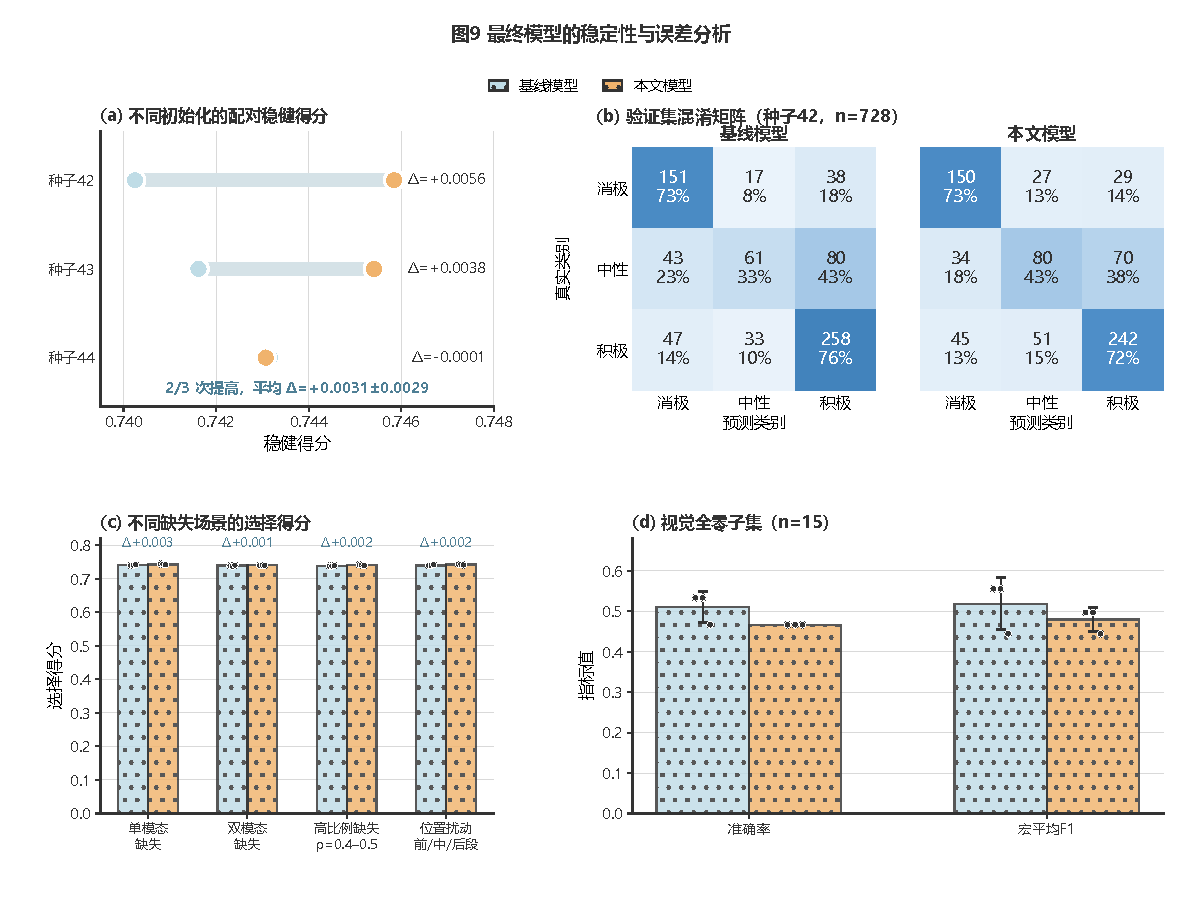
\includegraphics[width=1.0\textwidth]{figures/q2/fig13_q2_stability_error_analysis.pdf}
  \caption{最终模型的稳定性与误差分析。(a) 三个训练种子下与对应基线的配对鲁棒分数；(b) 种子42的干净验证集混淆矩阵，行为真实类别、列为预测类别；(c) 按缺失形式汇总的选择分数；(d) 15条视觉整段原生全零样本的分类准确率与宏平均F1。误差线表示三次训练种子的样本标准差，不表示置信区间。}
  \label{fig:fig13_q2_stability_error_analysis}
\end{figure}

\subsection{消融分析}\label{subsec:q2_ablation}
表~\ref{tab:q2_ablation} 压缩展示主要结构选择。更深的单模态时间编码器与训练阶段连续遮挡增强，在三次初始化的相同验证协议下均未超过基线。均值与最大值残差池化在一次初始化下有正向迹象，但缺少重复验证；低秩模态交互分支在同次初始化下降。跨模态重建的非零混合比例未在三次初始化中给出一致正收益；文本单独标准化下降，增大回归损失权重的收益很小且伴随准确率下降。可靠性加权分支有单次初始化的正向诊断，但没有同样完整的重复证据。因而本文保留参数开销较小、具有三次初始化配对结果的时间注意力残差池化方案。

\begin{table}[htbp]
\centering\small
\caption{主要结构与训练策略的验证集消融摘要。一次初始化结果仅为筛选证据，不与三次初始化均值作统计等同解释}
\label{tab:q2_ablation}
\begin{tabular}{@{}lccc@{}}
\toprule
方案 & 初始化次数 & 总参数量 & 综合鲁棒分数\\
\midrule
基线模型 & 3 & 163460 & $0.7417\pm0.0015$\\
单模态时间编码 & 3 & 957572 & $0.7351\pm0.0020$\\
基线加训练期连续遮挡 & 3 & 163460 & $0.7385\pm0.0025$\\
均值与最大值残差池化 & 1 & 163463 & $0.7443$\\
轻量时间注意力残差池化 & 3 & 164343 & $0.7448\pm0.0015$\\
\bottomrule
\end{tabular}
\end{table}

\FloatBarrier
\subsection{公开多模态模型对比}\label{subsec:q2_public_baselines}
表~\ref{tab:q2_public_baselines} 对比TFN、MulT、MISA与本文模型在附件2完整输入验证集上的三次初始化结果。三种公开模型均针对本题的aligned-50预计算特征作架构适配，并非对原论文训练流程的完全复现。公开模型按完整输入验证分数选择checkpoint，本文模型沿用固定缺失场景的综合鲁棒分数选择checkpoint，比较时须保留这一口径差异。

\begin{table}[htbp]
\centering\small\setlength{\tabcolsep}{4pt}
\caption{公开多模态模型在附件2完整输入验证集上的对比（三次初始化均值$\pm$样本标准差）}
\label{tab:q2_public_baselines}
\begin{tabular}{@{}lrcccc@{}}
\toprule
方法 & 参数量 & 准确率$\uparrow$ & 宏平均F1$\uparrow$ & MAE$\downarrow$ & 相关系数$\uparrow$\\
\midrule
TFN & 4,840,670 & $0.6099\pm0.0076$ & $0.5872\pm0.0083$ & $0.6336\pm0.0102$ & $0.6056\pm0.0098$\\
MulT & 624,094 & $0.6172\pm0.0148$ & $0.5891\pm0.0236$ & $0.6221\pm0.0260$ & $0.6369\pm0.0115$\\
MISA & 1,118,852 & $0.6131\pm0.0083$ & $0.6010\pm0.0060$ & $0.9175\pm0.1005$ & $0.6269\pm0.0087$\\
本文模型 & 164,343 & $0.6419\pm0.0057$ & $0.6241\pm0.0026$ & $0.6059\pm0.0066$ & $0.6472\pm0.0025$\\
\bottomrule
\end{tabular}
\end{table}


本文模型在准确率、宏平均F1和皮尔逊相关系数上取得更高均值，MAE均值更低，参数量也较少。MISA的MAE相对较高；已有检查确认其回归标签尺度、回归头输出和评价实现未发现错误，因此表中保留实际结果。

\FloatBarrier
\subsection{附件3专项测试集最终预测}\label{subsec:q2_attachment3}
附件3对齐版仅提供\texttt{text\_bert}、\texttt{audio}与\texttt{vision}，没有预计算的\texttt{text}特征。本文复用已验证的\texttt{text\_bert}$\rightarrow$\texttt{bert-base-uncased}$\rightarrow$\texttt{text[50,768]}接口适配：在20条同时具有原始文本特征与标记张量的已知样本上，604/604个有效行的余弦相似度最大值均位于同索引；特征最大绝对差为$3.0041\times10^{-5}$，RMSE为$8.3977\times10^{-7}$。同一锁定模型分别输入原特征与重构特征时，分类logit和回归输出的最大绝对差为$2.44\times10^{-6}$与$1.12\times10^{-6}$。模型参数未修改，也未重新训练。

表~\ref{tab:q2_attachment3_all} 列出全部30条附件3样本的最终预测。分类置信度为预测类别的softmax概率；表内不使用真实标签，也不据此调整模型。

\input{generated/table_q2_attachment3_all.tex}

预测类别中，消极7条（23.33\%）、中性11条（36.67\%）、积极12条（40.00\%）。预测情感强度均值为0.123114，样本标准差为0.611792，范围为$[-1.642545,1.539758]$；平均分类置信度为0.624599。附件3是无标签专项测试集，上述数值仅描述预测分布，不能计算准确率、宏平均F1、MAE或皮尔逊相关系数，也不能据此判断预测正确率。

\subsection{本问小结}
本问直接利用预计算特征，依靠有效位掩码防止填充进入池化，并以固定连续缺失场景检验预测模型。轻量时间注意力残差池化在宏平均F1、MAE及相关性上取得小幅平均收益，但准确率、个别双模态缺失条件及原生视觉全零子集仍有限制。下一问据此在同一预测函数上分析模型决策依据，而不把内部归因直接等同于真实媒体的因果解释。
\FloatBarrier
